%%%%%%%%%%%%%%%%%%%%%%%%%%%%%%%%%%%%%%%%%
% Stylish Article
% LaTeX Template
% Version 2.1 (1/10/15)
%
% This template has been downloaded from:
% http://www.LaTeXTemplates.com
%
% Original author:
% Mathias Legrand (legrand.mathias@gmail.com) 
% With extensive modifications by:
% Vel (vel@latextemplates.com)
%
% License:
% CC BY-NC-SA 3.0 (http://creativecommons.org/licenses/by-nc-sa/3.0/)
%
%%%%%%%%%%%%%%%%%%%%%%%%%%%%%%%%%%%%%%%%%

%-------------------------------------------------------------------------------------
%	PACKAGES 
%-------------------------------------------------------------------------------------

\documentclass[fleqn,11pt]{SelfArx} % Document font size and equations flushed left
\usepackage[francais]{babel} % Specify a different language here - english by default
\usepackage{hyperref}

\setlength{\columnsep}{0.55cm} % Distance between the two columns of text
\setlength{\fboxrule}{0.75pt} % Width of the border around the abstract
\definecolor{color1}{RGB}{0,0,90} % Color of the article title and sections
\definecolor{color2}{RGB}{0,20,20} % Color of the boxes behind the abstract and headings
\usepackage{hyperref} % Required for hyperlinks
\usepackage{xcolor}  
\usepackage{listings}
\usepackage{pdfpages}
\usepackage{amssymb}
%\usepackage[french]{babel}

\usepackage{courier} % Required for the courier font         
\hypersetup{hidelinks,colorlinks,breaklinks=true,urlcolor=blue,citecolor=color1,linkcolor=color1, bookmarksopen=false,pdftitle={Title},pdfauthor={Author}}

\providecommand\phantomsection{}


%--------------------------------------------------------------------------------------
%	CODE INCLUSION CONFIGURATION
%-------------------------------------------------------------------------------------
\usepackage{color}
 
\definecolor{codegreen}{rgb}{0,0.6,0}
\definecolor{codegray}{rgb}{0.5,0.5,0.5}
\definecolor{codepurple}{rgb}{0.58,0,0.82}
\definecolor{backcolour}{rgb}{0.95,0.95,0.92}
 
\lstdefinestyle{mystyle}{
    backgroundcolor=\color{backcolour},   
    commentstyle=\color{codegreen},
    keywordstyle=\color{magenta},
    numberstyle=\tiny\color{codegray},
    stringstyle=\color{codepurple},
    basicstyle=\footnotesize,
    breakatwhitespace=false,         
    breaklines=true,                 
    captionpos=b,                    
    keepspaces=true,                 
    numbers=left,                    
    numbersep=5pt,                  
    showspaces=false,                
    showstringspaces=false,
    showtabs=false,                  
    tabsize=2
}
 
\lstset{style=mystyle}



%-------------------------------------------------------------------------------------
%	INFORMATIONS
%-------------------------------------------------------------------------------------


\JournalInfo{Projet RESYS 2016-2017}
\Archive{Master 2 BIM-BMC, UPMC} 
\PaperTitle{Différenciation des précurseurs hématopoïétiques chez l'embryon}
\Authors{Nathalie Lehmann\textsuperscript{1}, Mariam Sissoko\textsuperscript{1} \\ Enseignants référents: \textbf{Hervé Isambert\textsuperscript{2}, Louis Verny\textsuperscript{2}, Nadir Sella\textsuperscript{2}}}

\affiliation{\textsuperscript{1}\textit{Master 2 Bioinformatique et Modélisation, Université Paris 6, France}}
\affiliation{\textsuperscript{2}\textit{Institut Curie, France}}


\Keywords{Réseaux de régulation -- Facteurs de transcription -- Hématopoïèse} 

\newcommand{\keywordname}{Mots-clés} % Defines the keywords heading name

%--------------------------------------------------------------------------------------
%	ABSTRACT
%--------------------------------------------------------------------------------------

\Abstract{Le but de ce projet de Master 2 de bioinformatique est de reconstruire le réseau de régulation régissant les expressions des facteurs de transcription clés pour la différenciation des précurseurs hématopoïétiques chez l'embryon. Dans cet objectif, nous avons d'abord procédé à un filtrage des données afin de garder les gènes d'intérêt, puis reconstruit des réseaux selon deux méthodes différentes : par clustering hierarchique et via l'algorithme polynomial PC\cite{pc} (\textit{Peter-Clark}). Enfin, en comparant nos résultats avec ceux présents dans la littérature scientifique, nous ferons état d'un modèle graphique simplifié expliquant les mécanismes impliquant la différenciation des cellules primitives en deux lignées distinctes hématopoïétique et endothéliale. Cette reconstruction de réseau a été effectuée à partir de données analysées par \textit{single cell RNA-seq} puis binarisées. }

 



%--------------------------DEBUT-------------------------------------

\begin{document}
\flushbottom % Makes all text pages the same height
\maketitle


\tableofcontents 

\thispagestyle{empty} 


%------------------------------------------------
%--------------INTRO----------------------------------
%------------------------------------------------
\section*{Introduction}
\addcontentsline{toc}{section}{Introduction}
Au cours du développement de l'embryon des Verté-brés, tous les tissus hématopoïétiques successivement actifs (foie, thymus, rate et moelle osseuse) sont colonisés par des cellules souches hématopoïétiques (CSH) d'origine extrinsèque. Le sac vitellin (SV) constitue l'unique exception à cette règle, puisque des CSH s'y développent in situ. Il a été observé que le SV constitue le premier site d'hématopoïèse de l'embryon\cite{Cumano} : c'est le lieu d'apparition des premières cellules sanguines propres à l'embryon. Cependant, de la lignée primitive à l'origine de celles-ci, émerge aussi les premières cellules endothéliales (constituant la paroi interne des vaisseaux sanguins). Dans ces conditions, quels sont les facteurs de transcription suffisants et/ou nécéssaires pour induire cette différenciation de la lignée primitive ?

\par Reconstruire le réseau de régulation contôlant cette différenciation pourrait permet de mieux appréhender les mécanismes de l'hématopoïèse primitive et de la formation des tissus sanguins. Or l'origine de certaines leucémies (ie l'anémie de Fanconi\cite{Fanconi}) reste encore difficile à déterminer, et l'établissement de tels réseaux pourrait alors favoriser la compréhension et l'établissement de protocoles expérimentaux très spécifiques. 
 
\par Il est important de spécifier que ce projet s'appuie largement sur l'article de Moignard et al., \textit{Decoding the regulatory network of early blood development from single-cell expression measurements}\cite{Moignard}. En effet, les données utilisées pour réaliser ce projet sont similaires à celles utilisées par les auteurs de l'article sus-nommé, et la démarche globale de reconstruction de réseau est relativement semblable, bien qu'allégrement simplifiée. 


%------------------------------------------------
%--------------METHODES----------------------------------
%------------------------------------------------

\section{Données et méthodes}


3 934 single cells - gene regulatory network
Data : niveau d'expresssion \\
Noeuds : gènes \\
Liens : interactions de régulation (activation ou inhibition) 
\subsection{Obtention du dataset}
Le dataset proposé rassemble les données d'expression binarisées de différents gènes pouvant soit avoir un rôle de régulation transcriptionnel, soit d'autres gènes marqueurs (\textit{housekeepers}). Les données étant binaires, le '1' représente un gène exprimé dans la condition correspondante, le '0' un gène non exprimé. 



\begin{figure}[ht]
\centering
\includegraphics[width=\linewidth]{images/debut2}
\caption{Processus de différenciation de la lignée primitive (PS) en 2 lignées distinctes : endothéliale (4SFG) et hématopoïétique (4SG)}
\label{fig:debut}
\end{figure}

Pour ceux qui souhaiteraient visualiser le cycle de développement embryonnaire murin de manière globale ainsi que les étapes critiques de l'hématopoïèse, les figures récapitulatives \ref{fig:devptCycle} et \ref{fig:devpt} sont accessibles dans la partie annexe. 


\subsubsection{scRNA-Seq}
Chaque type cellulaire se distingue par un profil d'expression de gènes bien spécifiques (bien que l'ADN soit le même). lorsque l'on veut étudier des phénomènes extrêmement précis ou que l'on est limité niveau quantité de matériel, les techniques traditionnelles révèlent leurs limites. Mais comme le disent les Shadoks, s'il n'y a pas de solution c'est qu'il n'y a pas de problème ! Et la solution ici tient en trois mots : Single Cell Sequencing. Cette technique apporte avec elle son lot de complications, néanmoins le single-cell sequencing permet une analyse génomique et transcriptomique à l'échelle d'une seule cellule et permet d'affiner encore et toujours plus nos connaissances. Avec ce procédé, il devient possible d'estimer la variabilité intra-tissulaire, d'étudier des stades embryonnaires précoces, de décortiquer la composition des tumeurs ou même encore de retracer les lignées cellulaires au cours du développement (source : \href{http://bioinfo-fr.net/single-cell-sequencing?hilite=single+cell+RNA-seq}{bioinfo-fr} )\footnote{http://bioinfo-fr.net}. 

lmites : En effet, vu que l'on part avec une quantité réduite d'ARN (ou ADN), deux étapes d'amplification sont nécessaires (au lieu d'une seule normalement). L'amplification peut créer des biais dans vos données et il est important d'en avoir conscience, surtout quand on fait du single-cell. D'ailleurs, à cause de ces bruits générés par une grosse amplification, il va être difficile d'analyser de manière très fine l'expression de gènes faiblement exprimés.

Le second souci du single-cell, c'est la  variabilité de l'expression entre les cellules, même de type identique. De prime abord, on pourrait s'attendre à avoir des profils d'expression assez similaires d'une cellule à une autre, surtout quand il s'agit du même type. Or, il faut savoir que ce n'est pas tout à fait le cas. Si vous savez que parmi vos cellules il y a plusieurs types cellulaires, mais vous ne savez pas qui est quoi, vous devrez passer par une étape de sélection d'un set de gènes que vous savez plus ou moins spécifiques à tel ou tel type cellulaire. Vous pourrez ensuite procéder à un clustering hiérarchique (et/ou ACP) de vos échantillons pour les classer en fonction de la manière dont elles expriment ces gènes. Si vous vous lancez dans ce type d'analyses sans sélectionner au préalable un set de gènes, il y a peu de chance que vous réussissiez à classer correctement vos cellules.

\subsubsection{Binarisation des données}



\subsection{Filtre des données}
Afin d'obtenir un set de données non biaisées, nous avons choisi d'appliquer un filtre afin d'éliminer les gènes exprimés dans 100\% des cas (codé en Python, on ôte du dataset les colonnes où il n'exsite que des '1'). Les gènes qui disparaissent alors sont référencés ci-dessous, et leur fonction en tant que "housekeeper" a été vérifiée via le site de la \href{https://www.ncbi.nlm.nih.gov/gene}{NCBI}\footnote{https://www.ncbi.nlm.nih.gov/gene} / ou via mouse genom database :
\begin{itemize}
\item \textbf{Eif2b1}
\item \textbf{Mrpl19}
\item \textbf{Polr2a}
\item \textbf{Ubc} 
\end{itemize}
Dire qu'on a pensé à établir un seuil mais pas la peine. 

\subsection{Gènes d'intérêt}
Expliquer tous les datasets formés : par lignée (fonctionnel) ou par type cellulaire (temporel). 

%The homeobox genes encode a highly conserved family of transcription factors that play an important role in morphogenesis in all multicellular organisms. Mammals possess four similar homeobox gene clusters, HOXA, HOXB, HOXC and HOXD, located on different chromosomes, consisting of 9 to 11 genes arranged in tandem.  (wiki)

\subsection{Reconstruction de réseaux}
Noeud = gène \\
Lien = relation entre les gènes (activation ou inhibition). 
\subsubsection{Algorithme PC}
MIIC = Multivariate Information based Inductive Causation
Interface cytoscape via Miic Web Server.  \\
miic aims at reconstructing causal, non-causal or mixed networks between the variables of your dataset and is suitable for either categorical or quantitative discrete variables. \\
Default value: −1 means that all the samples are taken as independent observations given the common experi- mental conditions \\
Complexity : Complexity criterion for the network reconstruction (NML: Normalized Maximum Likelihood; MDL / BIC: Minimum Description Length / Bayesian Information Criterion). Default value: NML \\
Orientation : Is the orientation of v-structures enabled ? \\
Propagation : Should orientation be propagated downstream of v-structures ? (see main text). \\
Latent : When enabled, this parameter allows to detect the effects of unobserved latent causes on the relationships between observed variables (i.e. bidirected edges, see main text).

Confidence plot : An Igraph-based plot of the network, where the color of the edges is scaled on their confidence.
Correlation plot : An Igraph-based plot of the network, where edges’ color is scaled on their partial correlation coefficient.

PC : Algorithme polynomial pour l'inférence de structure de graphe. 

\begin{figure}[ht]
\centering
\includegraphics[width=\linewidth]{images/pc}
\caption{Algorithme PC}
\label{fig:pcd}
\end{figure}


\subsubsection{Réseau hierarchique}
Code R. 

%------------------------------------------------
%--------------RESULTATS----------------------------------
%------------------------------------------------


\section{Résultats et discussion}
Faire un choix entre précision (spécificité des données ?) et lisibilité. 
\subsection{Réseaux obtenus}
Face à la diversité des paramètres qui peuvent être modifiés via MIIC (sur l'interface Cytoscape), nous avons choisi de ne nous focaliser que sur un unique paramètre : le seuil de confiance. Ainsi nous avons construit, pour chaque set de données généré, de 2 à 10 réseaux différents, les premiers réseaux ayant un seuil de confiance élevé (par rapport à l'étendue de celui-ci) et les derniers ayant un seuil de confiance plus bas. Le nombre de réseau obtenu est fonction du nombre de gènes compris dans le dataset. Tous les autres paramètres par défaut sont restés inchangés par souci de compréhension. 
% On aurait pu aussi choisir de modifier le confidence cut This step aims at filtering the network according to a confidence ratio, calculated by estimating the probability to discard an edge in more randomization of the input dataset and comparing it to the estimation of the probability in the real dataset. The closer this ratio is to 0, the more trustworthy the edge is.


%Cependant, nous avons testé quelques dataset en modifiant la latence (par défaut : prise en compte) afin de voir si des différences notables quant aux relations entre les noeuds apparaissaient.

Il faut prendre en compte que plus le seuil de confiance est élevé, moins les relations sont nombreuses, donc des gènes disparaissent du réseau ainsi formé. Cependant, ces relations restantes sont d'autant plus fiables. 

\subsection{Similarité des réseaux obtenus avec ceux de la littérature}
\begin{figure*}[ht]
\centering
\includegraphics[width=\linewidth]{results/filtre33}
\caption{Résultats obtenus avec un seuil de confiance de ? }
\label{fig:filtre33}
\end{figure*}

\begin{figure}[ht]
\centering
\includegraphics[width=\linewidth]{results/filtre33prof}
\caption{Résultats issus de \textit{Verny et al. submitted} (dans le cours de RESYS)}
\label{fig:filtre33}
\end{figure}


\begin{figure*}[ht]
\centering
\includegraphics[width=\linewidth]{results/arbre1}
\caption{Arbre obtenu par clustering hierarchique non supervisé - 42 gènes}
\label{fig:arbre1}
\end{figure*}

\begin{figure*}[ht]
\centering
\includegraphics[width=\linewidth]{results/arbre33genes}
\caption{Arbre obtenu par clustering hierarchique non supervisé - 33 gènes}
\label{fig:arbre33}
\end{figure*}


\subsection{Vérifications expérimentales}

\begin{figure}[ht]
\centering
\includegraphics[width=\linewidth]{images/ikarosNotchGata}
\caption{ikaros - Notch - Gata}
\label{fig:ikarosNotchGata}
\end{figure}


\begin{figure*}[ht]
\centering
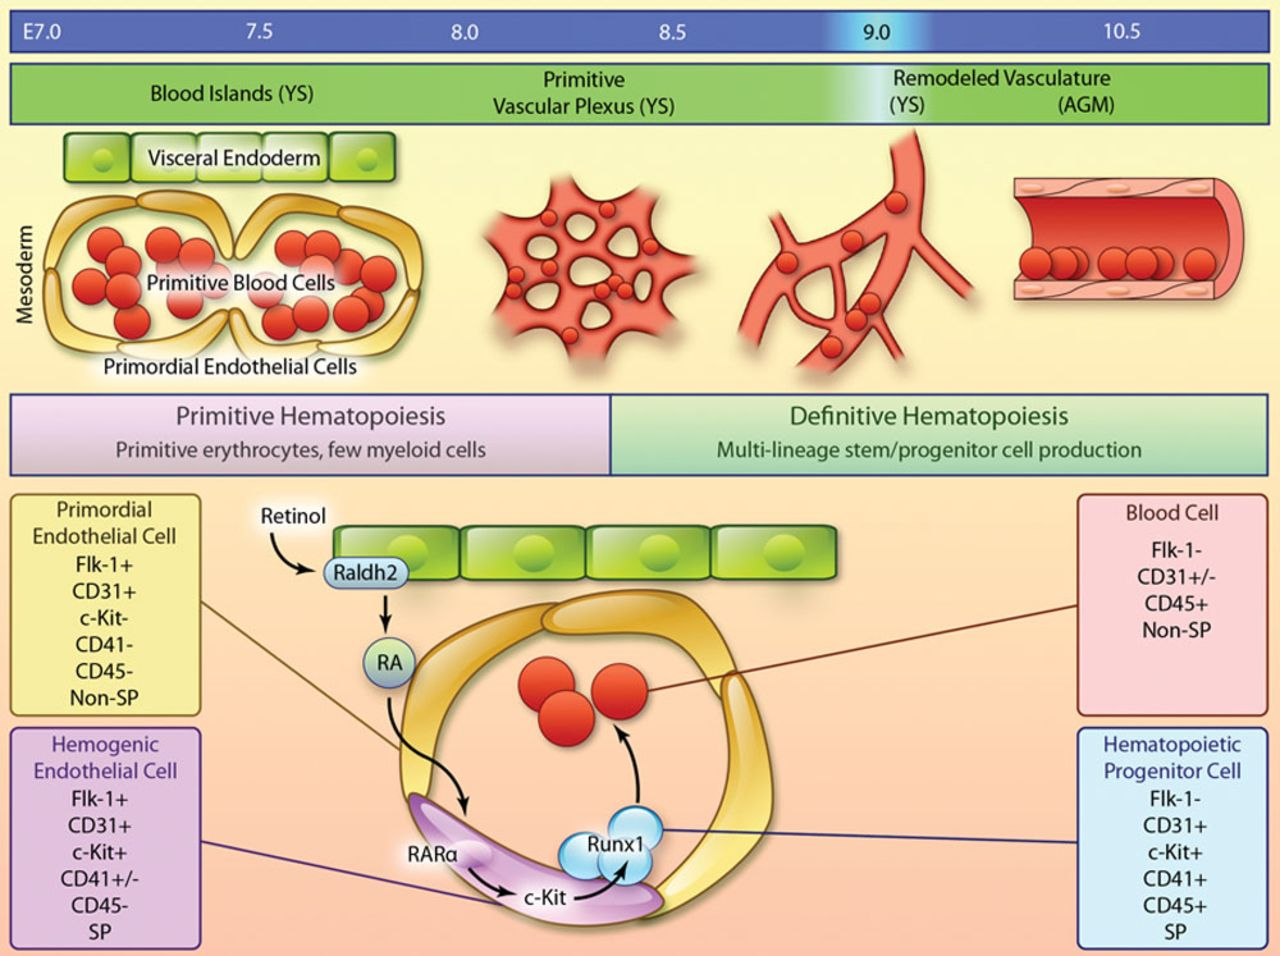
\includegraphics[width=\linewidth]{images/synthese}
\caption{Hematopoiese}
\label{fig:synthese}
\end{figure*}


%\begin{figure}[ht]
%\centering
%\includegraphics[width=\linewidth]{images/ResultsPDB}
%\caption{Affichage via PyMol du meilleur résultat du docking. L'Agest en violet, tandis que l'Ac est en vert et bleu (chaînes lourde et légère)}
%\label{fig:ResultsPDB}
%\end{figure}


%------------------------------------------------
%--------------CONCLUSION----------------------------------
%------------------------------------------------

\section*{Conclusion}
\addcontentsline{toc}{section}{Conclusion}



%------------------------------------------------
\newpage
\phantomsection
\bibliographystyle{unsrt}
\bibliography{sample}

\newpage
\section*{Annexes}

\begin{figure*}[ht]
\centering
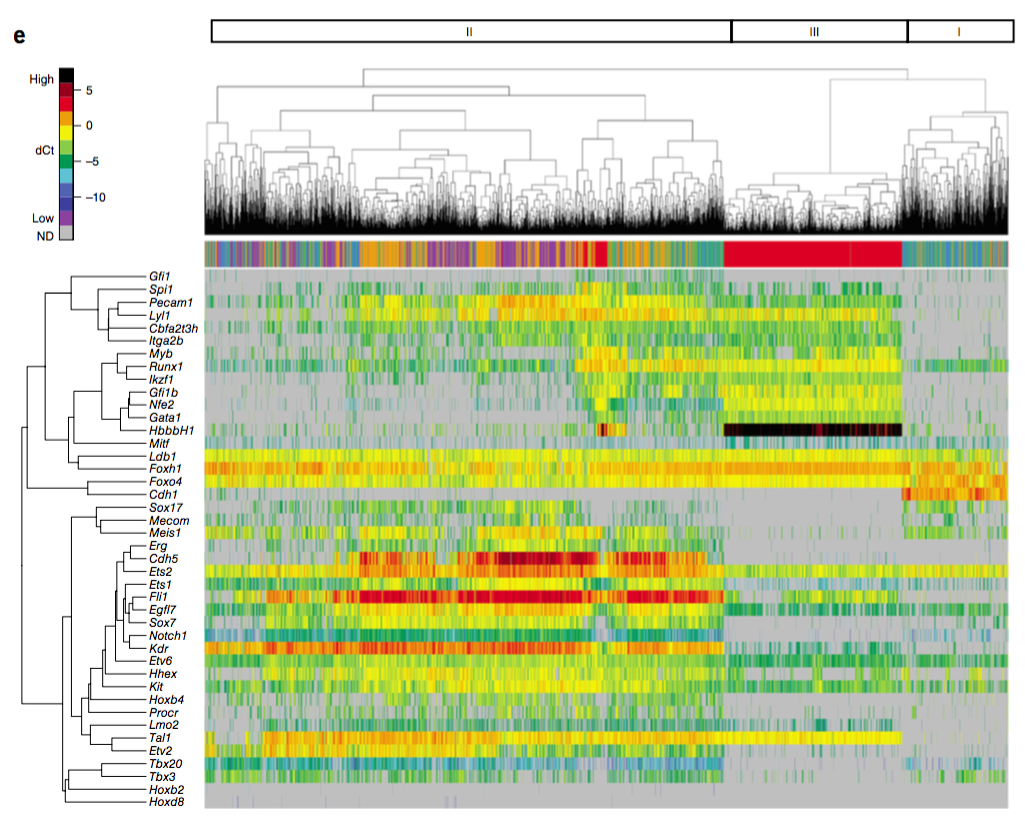
\includegraphics[width=\linewidth]{images/article2}
\caption{Résultats de... ? issus de \textit{Moignard et al.}}
\label{fig:artcile2}
\end{figure*}

\begin{figure*}[ht]
\centering
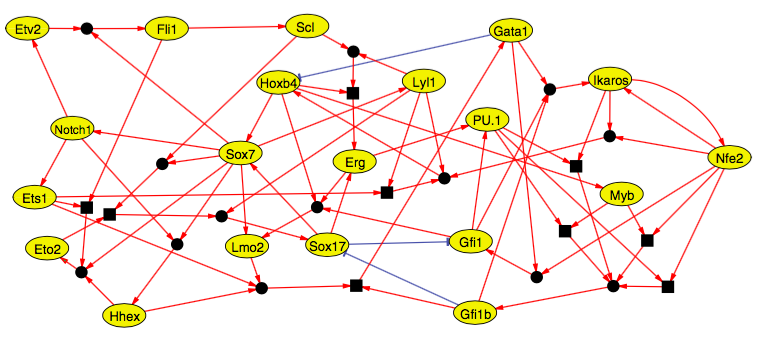
\includegraphics[width=\linewidth]{images/article3}
\caption{Graphe orienté issus de \textit{Moignard et al.}}
\label{fig:artcile2}
\end{figure*}

\begin{figure*}[ht]
\centering
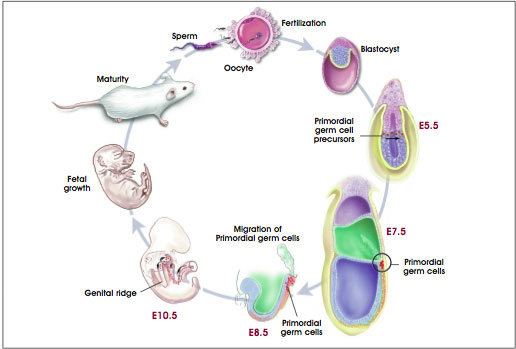
\includegraphics[width=\linewidth]{images/devptCycle}
\caption{Cycle de développement de \textit{Mus musculus}}
\label{fig:devptCycle}
\end{figure*}

\begin{figure*}[ht]
\centering
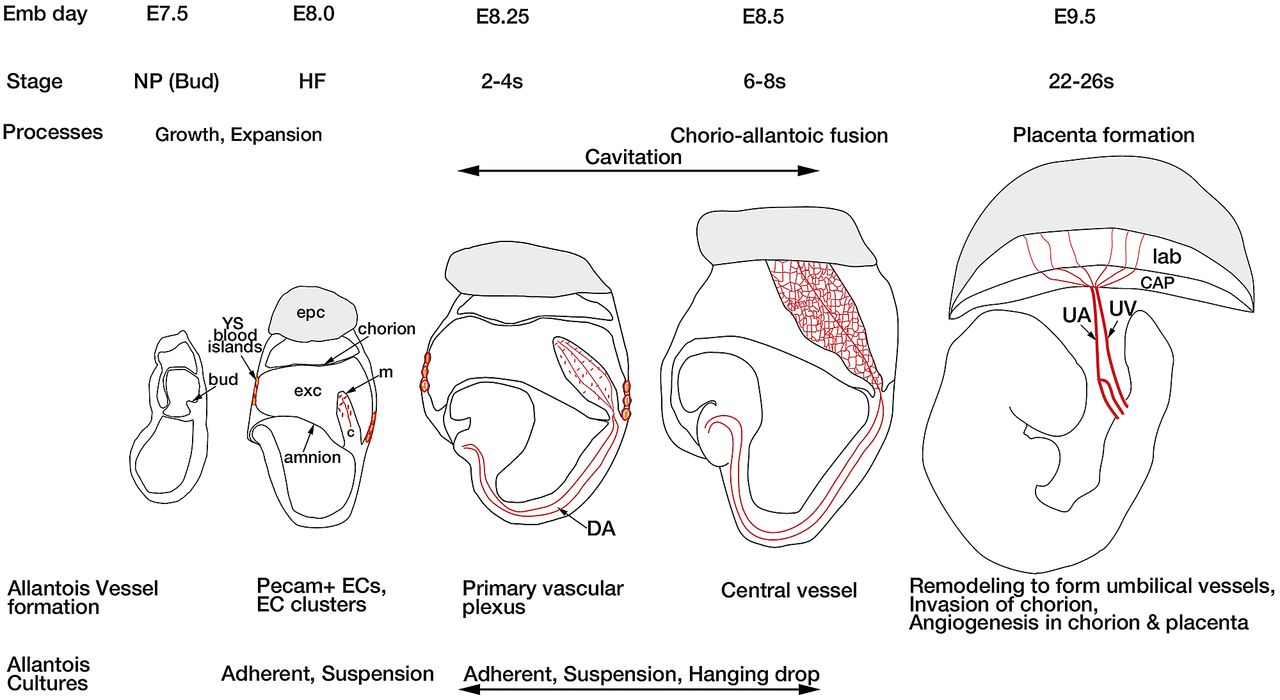
\includegraphics[width=\linewidth]{images/devpt}
\caption{Détails du développement de \textit{Mus musculus}\cite{Gaudin} du stade E7 à E11.5, dans le compartiment extra-embryonnaire (en rouge) et intra-embryonnaire (en jaune). En encart figurent les sites impliqués dans la génération des CSH, c’est-à-dire l’aorte et sa partie ventrale (et les artères omphalomésentérique (OA) et ombilicale (UA)). AGM : aorte-gonades-mésonephros ; FF : foie fœtal ; P-Sp : splanchnopleure para-aortique ; Sp : splanchnopleure ; SV : sac vitellin}
\label{fig:devpt}
\end{figure*}




%\section*{Annexes}

 
%\addcontentsline{toc}{section}{Annexes}
%
%\subsection*{Matériel additionnel} 
%\addcontentsline{toc}{subsection}{Matériel additionnel}
%\subsubsection{Filtres}
%\subsubsection{Fonction de score}

%\begin{figure}[ht]\centering
%\includegraphics[width=\linewidth]{images/poidsScoring}
%\caption{Poids utilisés pour les fonctions de score (utilisés dans RosettaDock\cite{rosettaDOCK}, pour le scoring de haute définition)}
%\label{fig:poidsScoring}
%\end{figure}



%\subsection*{Chronologie du docking}
%\addcontentsline{toc}{subsection}{Chronologie du docking}
%
%\subsection*{Outils de docking}
%\addcontentsline{toc}{subsection}{Outils de docking}


%----------------------------------------------------------------------------------------
%	REFERENCE LIST
%----------------------------------------------------------------------------------------

%----------------------------------------------------------------------------------------

\end{document}






%Articles de réf\cite{Pedotti}
%ref\cite{Rajkannan}
%ref\cite{Sela-Culang}
%ref\cite{Kuroda}
%ref\cite{Krawczyk}
%ref\cite{Abhinandan}
%ref\cite{Gabb}
%\cite{proABC}

%\url{http://www.wikibooks.org}


% Reference to Figure \ref{fig:results}.

%\begin{description}
%\item[Word] Definition
%\item[Concept] Explanation
%\item[Idea] Text
%\end{description}


%\begin{figure*}[ht]\centering % Using \begin{figure*} makes the figure take up the entire width of the page
%\includegraphics[width=\linewidth]{view}
%\caption{Wide Picture}
%\label{fig:view}
%\end{figure*}
%
%\lipsum[4] % Dummy text
%
%\begin{equation}
%\cos^3 \theta =\frac{1}{4}\cos\theta+\frac{3}{4}\cos 3\theta
%\label{eq:refname2}
%\end{equation}
%
%\lipsum[5] % Dummy text
%
%\begin{enumerate}[noitemsep] % [noitemsep] removes whitespace between the items for a compact look
%\item First item in a list
%\item Second item in a list
%\item Third item in a list
%\end{enumerate}
%
%\subsection{Subsection}
%
%\lipsum[6] % Dummy text
%
%\paragraph{Paragraph} \lipsum[7] % Dummy text
%\paragraph{Paragraph} \lipsum[8] % Dummy text
%
%\subsection{Subsection}
%
%\lipsum[9] % Dummy text
%
%\begin{figure}[ht]\centering
%\includegraphics[width=\linewidth]{results}
%\caption{In-text Picture}
%\label{fig:results}
%\end{figure}
%

%\begin{table}[hbt]
%\caption{Table of Grades}
%\centering
%\begin{tabular}{llr}
%\toprule
%\multicolumn{2}{c}{Name} \\
%\cmidrule(r){1-2}
%First name & Last Name & Grade \\
%\midrule
%John & Doe & $7.5$ \\
%Richard & Miles & $2$ \\
%\bottomrule
%\end{tabular}
%\label{tab:label}
%\end{table}

%\footnote{And some mathematics $\cos\pi=-1$ and $\alpha$ in the text.}.
